\documentclass[titlepage]{article}
\usepackage[utf8]{inputenc}

\title{
  \textbf{Dokumentacja} \\
  System do zarządzania boiskiem szkolnym}
\date{January 2021}

\author{Develop Team}
\usepackage{natbib}
\usepackage[T1]{fontenc}
\usepackage{graphicx}
\usepackage{polski}
\usepackage{indentfirst}
\usepackage{sectsty}
\usepackage{hyperref}




\begin{document}

\maketitle
\tableofcontents
\section*{Wstęp}
\addcontentsline{toc}{section}{Wstęp}

Głównym założeniem tej aplikacji jest rezerwowane boiska za pomocą strony internetowej. Zapewnia nam ona logowanie poprzez CAS. Cały projekt składa się z 
\begin{itemize}
  \item Aplikacji Bacekndowej opatej o Node.js
  \item Aplikacji frontendowej opartej o React.js
  \item Aplikacji frontendowej (administrator) opartej o ReactAdmin.js
\end{itemize}

Aplikacja korzysta z architektury REST oraz jest dostosowana do urządzeń mobilnych

\newpage
\section{Backend}

\begin{figure}[h]
\centering
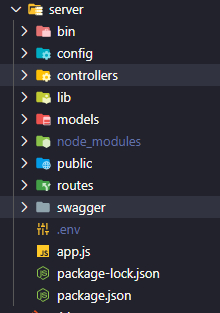
\includegraphics[width=0.5\textwidth]{struktura.png}
\caption{Struktura backendu}
\label{fig:obrazek struktura}
\end{figure}

\indent Część backendu w aplikacji do zarządzania boiskiem szkolnym jest napisany w języku JavaScript oparta o framework Express.js.


\subsection{Katalog config}
W tym katalogu mieszczą się dwa pliki
\begin{figure}[h]
\centering
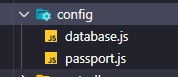
\includegraphics[width=0.5\textwidth]{config.png}
\caption{config katalog}
\label{fig:obrazek config}
\end{figure}
\subsubsection{database.js}
Ustawiamy z której bazy danych chcemy korzystać. Ustala się to zmienną NODE\_ENV w pliku .env
\subsubsection{passport.js}
Zawierają się tam wszystkie ustawienia od autoryzacji użytkownika (CAS oraz logowanie niezależne)

\subsection{Katalog controllers}
Katalog zawiera pliki które zawierają funkcje służące do działania całej aplikacji, są one eksportowane i podpinane pod ścieżki w folderze routes

\begin{figure}[h]
\centering
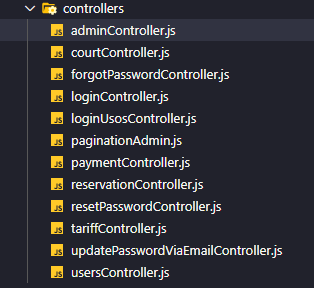
\includegraphics[width=0.5\textwidth]{controllers.png}
\caption{controllers katalog}
\label{fig:obrazek controllers}
\end{figure}

\subsubsection{adminController.js}
Plik ten zawiera wszystkie funkcje, potrzebne to zarządzania aplikacją frontedową przez administratora systemu. 

\subsubsection{courtController.js}
Tworzymy tutaj rozkład boiska który chcemy aby był dostępny dla naszych klientów

\subsubsection{forgotPasswordController.js}
Funkcje odpowiedzialne za przypominanie hasła

\subsubsection{loginController.js}
Logowanie i wylogowywanie użytkownika z aplikacji (outh)

\subsubsection{loginUsosController.js}
Logowanie i wylogowywanie użytkownika z aplikacji (CAS) \\
Link do dokuemntacji: \url{https://apps.usos.edu.pl/developers/api/}

\subsubsection{paginationAdmin.js}
Middleware do aplikacji adminstratora pomagające ustalić podział rekordów na strony

\subsubsection{paymentController.js}
Metody odpowiedzialne za wytworzenie tokenu w serwisie Pay'u oraz dokonanie płatności

\subsubsection{reservationController.js}
Controller odpowiedzialny za tworzenie rezerwacji, modyfikacji, usuwania.

\subsubsection{resetPasswordController.js}
Sprawdzenie czy możemy ustawić nowe hasło

\subsubsection{tariffController.js}
Dodawanie, modyfikowanie i usuwanie cennika obiektu

\subsubsection{updatePasswordViaEmailController.js}
Controller do wygenerowania nowego hasła

\subsubsection{usersController.js}
Tworzymy nowego użytkownika oraz modyfikujemy jego dane personalne








\end{document}
